\begin{recipe}
    [% 
        preparationtime = {\unit[30]{min}},
        portion = {\portion{2}},
        bakingtime = {\unit[25]{min}}
    ]
    {Trout on vegetables slices}
    \introduction{%
        I think that a well seasoned fresh fish is the most festive dish.
        Add sliced vegetables and pesto to make it more special.
    }

    \ingredients[17]{%
        2 & fresh trout \\
        \unit[2]{tbs.} & Butter \\
        4 & Lemon slices \\
        & Coriander powder \\
        3 & Squeezed garlic cloves \\
        4 & Potatoes \\
        2 & Beetroot (raw!) \\
        & Thyme \\
        4 hfl. & Green leaves* \\
        2 tbs. & Yeast flakes \\
        4 & Garlic cloves \\
        \nicefrac{1}{4} c. & Roast pumpkin seeds \\
        4 tbs. & Olive oil \\
        & Lemon juice
    }

    \preparation{%
        \step Slice (very finely) peeled beetroot and potatoes.
        Blanch potatoes for 5-7 min.
        
        \step In a mortar, grind: coriander, salt, pepper and garlic.
        Add butter and mix.
        
        \step Wash trout and stuff with mixture from the mortar; add lemon slices.
        
        \step Line a tray with aluminium foil, leaving free foil to cover trout later on.
        Layer potatoes (sprinkle with olive oil and thyme) and beetroot.
        
        \step Place trout on vegetables, cover tightly with foil. \underline{Bake at \unit[180]{\textcelcius} for 20-25 min.}
        
        \step \textbf{Pesto:} Blend leaves, garlic, seeds, oil, yeast flake, lemon juice and salt.
        
        \step Serve trout as follows: on the plate layer vegetables, in the middle spread pesto, place rout on the pesto.
    }

    \hint{%
        *Green leaves: in Poland I would normally use either radish leaves or kohlrabi or mixture of both.
        However, I'm aware that if you don't have an allotment you may not be able to buy them in the UK.
        Good alternative will be fresh parsley or carrot top.
    }

\end{recipe}

\begin{figure}[h]
    \centering
    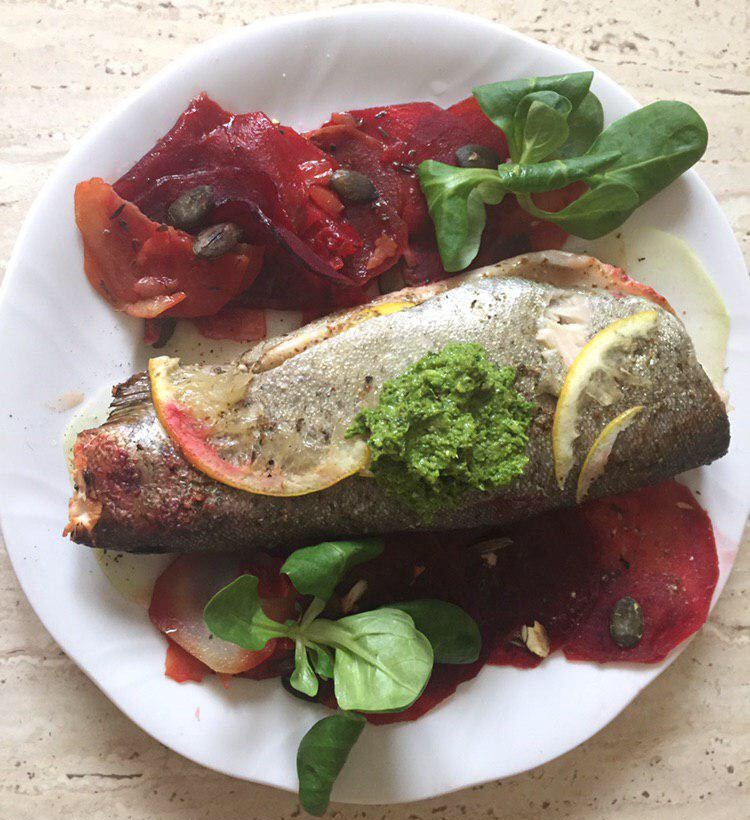
\includegraphics[height=11cm]{pic/trout}
\end{figure}
\begin{figure}[h]
    \centering
    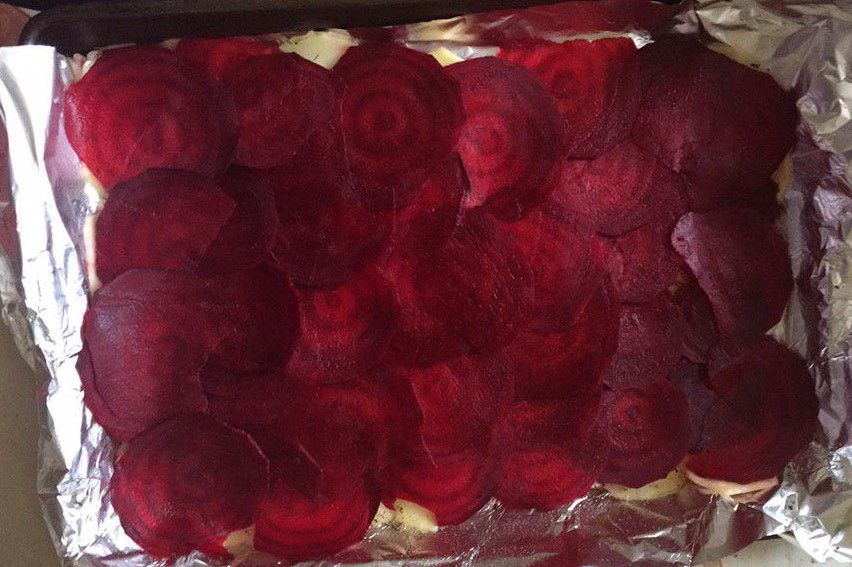
\includegraphics[height=8cm,angle=0]{pic/beetroot}
\end{figure}
% TODO: put images side to side
